% Options for packages loaded elsewhere
\PassOptionsToPackage{unicode}{hyperref}
\PassOptionsToPackage{hyphens}{url}
%
\documentclass[
]{article}
\usepackage{lmodern}
\usepackage{amssymb,amsmath}
\usepackage{ifxetex,ifluatex}
\ifnum 0\ifxetex 1\fi\ifluatex 1\fi=0 % if pdftex
  \usepackage[T1]{fontenc}
  \usepackage[utf8]{inputenc}
  \usepackage{textcomp} % provide euro and other symbols
\else % if luatex or xetex
  \usepackage{unicode-math}
  \defaultfontfeatures{Scale=MatchLowercase}
  \defaultfontfeatures[\rmfamily]{Ligatures=TeX,Scale=1}
\fi
% Use upquote if available, for straight quotes in verbatim environments
\IfFileExists{upquote.sty}{\usepackage{upquote}}{}
\IfFileExists{microtype.sty}{% use microtype if available
  \usepackage[]{microtype}
  \UseMicrotypeSet[protrusion]{basicmath} % disable protrusion for tt fonts
}{}
\makeatletter
\@ifundefined{KOMAClassName}{% if non-KOMA class
  \IfFileExists{parskip.sty}{%
    \usepackage{parskip}
  }{% else
    \setlength{\parindent}{0pt}
    \setlength{\parskip}{6pt plus 2pt minus 1pt}}
}{% if KOMA class
  \KOMAoptions{parskip=half}}
\makeatother
\usepackage{xcolor}
\IfFileExists{xurl.sty}{\usepackage{xurl}}{} % add URL line breaks if available
\IfFileExists{bookmark.sty}{\usepackage{bookmark}}{\usepackage{hyperref}}
\hypersetup{
  hidelinks,
  pdfcreator={LaTeX via pandoc}}
\urlstyle{same} % disable monospaced font for URLs
\usepackage{graphicx}
\makeatletter
\def\maxwidth{\ifdim\Gin@nat@width>\linewidth\linewidth\else\Gin@nat@width\fi}
\def\maxheight{\ifdim\Gin@nat@height>\textheight\textheight\else\Gin@nat@height\fi}
\makeatother
% Scale images if necessary, so that they will not overflow the page
% margins by default, and it is still possible to overwrite the defaults
% using explicit options in \includegraphics[width, height, ...]{}
\setkeys{Gin}{width=\maxwidth,height=\maxheight,keepaspectratio}
% Set default figure placement to htbp
\makeatletter
\def\fps@figure{htbp}
\makeatother
\setlength{\emergencystretch}{3em} % prevent overfull lines
\providecommand{\tightlist}{%
  \setlength{\itemsep}{0pt}\setlength{\parskip}{0pt}}
\setcounter{secnumdepth}{-\maxdimen} % remove section numbering
\ifluatex
  \usepackage{selnolig}  % disable illegal ligatures
\fi

\author{}
\date{}

\begin{document}

\hypertarget{counting}{%
\section{Counting}\label{counting}}

\hypertarget{lists}{%
\subsection{Lists}\label{lists}}

\textbf{Definition:} a (finite) list is an element of the Cartesian
product of sets \(X=X_1\times\cdots X_n\). A common counting problem is
to determine the number of lists with certain properties whose entries
are drawn from a Cartesian product like \(X\).

\hypertarget{multiplication-principle}{%
\subsection{Multiplication Principle}\label{multiplication-principle}}

\begin{figure}
\centering
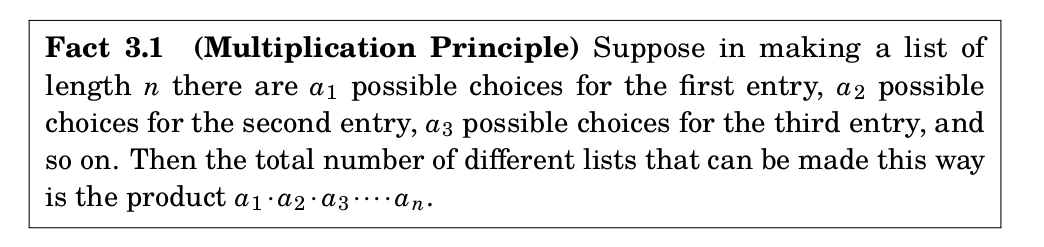
\includegraphics{../../png/MultiplicationPrinciple.png}
\caption{Multipication Principle (p.~69)}
\end{figure}

This informal principle can be applied in many settings, although in
most cases there is a \emph{hidden} proof by induction.

\hypertarget{example}{%
\subsection{Example}\label{example}}

\textbf{Proposition:} Suppose that \(X_1,\ldots,X_n\) are finite sets.
Then \[
|X_{1}\times\cdots\times X_{n}|=|X_{1}||X_{2}|\cdots |X_{n}|.
\] \vfill\eject

\hypertarget{example-1}{%
\subsection{Example}\label{example-1}}

How many ways can you order a coffee if your choices are whole, skim, or
soy milk; small, medium, or large size; and one or two shots of
espresso?

\vfill\eject

\hypertarget{example-2}{%
\subsection{Example}\label{example-2}}

Consider lists of length \(4\) made with the symbols \(A,B,C,D,E,F,G\).

\textbf{Question:} How many lists are there made up of these symbols (no
special conditions)

\vfill\eject

\hypertarget{example-continued}{%
\subsection{Example continued}\label{example-continued}}

\textbf{Question:} How many lists are there if no letter is repeated?

\vfill\eject

\hypertarget{example-continued-1}{%
\subsection{Example continued}\label{example-continued-1}}

\textbf{Question:} How many lists are there if there are no repetitions,
and at least one of the letters is an \(E\)?

\vfill\eject

\hypertarget{example-continued-2}{%
\subsection{Example continued}\label{example-continued-2}}

\textbf{Question:} How many lists are there if repetition \emph{is}
allowed, and the list contains at least one \(E\)?

\end{document}
